%\documentclass[handout]{beamer}
%\documentclass[14pt]{beamer}
\documentclass{beamer}

\usepackage[english]{babel}
\usepackage[utf8]{inputenc}
\usepackage{multirow}
\usepackage{booktabs}
\usepackage{amsmath}
\usepackage{amssymb}
\usepackage{subfigure}
\usepackage{color}
\usepackage{graphicx}
\definecolor{blue}{RGB}{000, 103, 198}
\definecolor{green}{HTML}{249140}
\definecolor{red}{HTML}{c71712}
\usepackage{colortbl}
\usepackage{tikz}
\usepackage{pgfplots}
\pgfplotsset{compat=1.5.1}

\bibliographystyle{apalike}

\usetikzlibrary{decorations.pathreplacing}
\usetikzlibrary{intersections}
\usetikzlibrary{shapes,snakes}

\usecolortheme[RGB={000, 103, 198}]{structure}
\setbeamertemplate{footline}[frame number]
\setbeamertemplate{navigation symbols}{}

\colorlet{darkgreen}{green}
\colorlet{darkred}{red}

\renewcommand<>{\alert}[1]{{\color#2{darkred}#1}}
\newcommand<>{\alertg}[1]{{\color#2{darkgreen}#1}}
\newcommand<>{\alertb}[1]{{\color#2{blue}#1}}

\title{ARCH-COMP Category Report:\\ Continuous and Hybrid Systems with 
Nonlinear Dynamics}

\author{
  Fabian Immler,
  Matthias Althoff,
  Luis Benet,
  Alexandre Chapoutot,
  Xin Chen,
  Marcelo Forets,
  Luca Geretti, Niklas Kochdumper, David P.Sanders, Christian Schilling}
\institute{
  Carnegie Mellon University (USA),
  ENSTA ParisTech (France),
  IST Austria (Austria),
  Technische Universit\"at M\"unchen (Germany),
  Univ. Grenoble Alpes (France),
  Universidad Nacional Aut\'onoma de M\'exico, (Mexico),
  University of Dayton (USA), 
  University of Illinois at Urbana-Champaign (USA),
  University of Verona (Italy),
}
\AtBeginSection[]{
  \begin{frame}
  \vfill
  \centering
  \begin{beamercolorbox}[sep=8pt,center,shadow=true,rounded=true]{title}
    \usebeamerfont{title}\insertsectionhead\par%
  \end{beamercolorbox}
  \vfill
\end{frame}
}

\begin{document}

\frame{\thispagestyle{empty}\titlepage}

\section{Tools}

\begin{frame}{Tools}

\begin{block}{since 2017}
\begin{itemize}
  \item \textbf{CORA}: zonotopes, linearization / \alert<3>{polynomial zonotopes}
  \item \textbf{Flow*}:\\
  continuous reachability: \alert<3>{Taylor Models}, symbolic remainders \\
  discrete jumps: domain contraction, range overapproximation, box/parallelotope aggregation
  \item \textbf{Isabelle/HOL}: formally verified (performance secondary) \\
  zonotopes, \alert<4>{affine arithmetic, Runge-Kutta methods}
\end{itemize}
\end{block}

\uncover<+(1)->{
  \begin{block}{New 2019}
  \begin{itemize}
    \item \textbf{Ariadne}: based on \emph{Computable Analysis}
    \item \textbf{DynIbex}: interval constraint propagation,
      \alert<4>{affine arithmetic, Runge-Kutta methods}
    \item \textbf{JuliaReach}: \alert<3>{Taylor Models}
  \end{itemize}
  \end{block}
}
\end{frame}

\begin{frame}{Tools missing from 2018}
\begin{itemize}
  \item \textbf{C2E2}: busy
  \item \textbf{CORA/SX}: busy
  \item \textbf{SymReach}: major updates for next year?
\end{itemize}
\end{frame}


\section{Benchmarks}

\begin{frame}{Benchmarks}
\begin{itemize}
	\item same problems as last year
  \item added parameters for more fine-grained overview of the capabilities of the different algorithms and tools
  \item parameter for stiffness in van-der Pol
  \item more initial sets for Laub-Loomis
\end{itemize}
\end{frame}

\begin{frame}{van der Pol}
\[
\left\{
\begin{array}{lcl}
\dot{x} & = & y \\
\dot{y} & = & \mu(1 - x^2) y - x
\end{array}
\right.
\]
{\Huge {\color{green}$\mu = 1$}} (from last year),\\
{\Huge {\color{blue}$\mu = 2$}} (harder!)\\
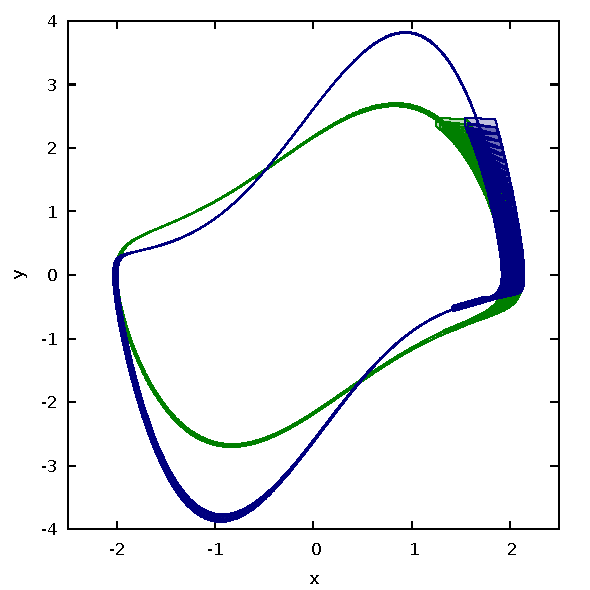
\includegraphics[width=5.5cm, height=5.5cm]{../results_Isabelle/out_vdp.pdf}
\end{frame}

\begin{frame}{van der Pol}
\begin{columns}
  \column{5.5cm}
  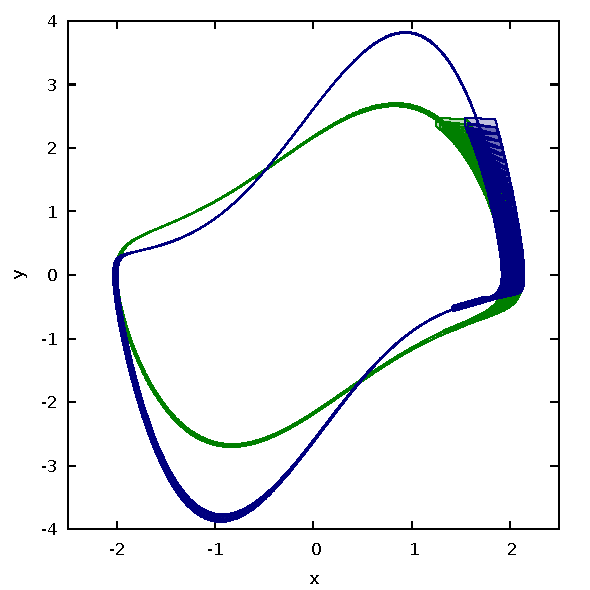
\includegraphics[width=5.5cm, height=5.5cm]{../results_Isabelle/out_vdp.pdf}
  \column{5.5cm}
  \begin{itemize}
    \item Pseudo-Invariants
    \begin{itemize}
      \item manual interaction
      \item more for $\mu = 2$
    \end{itemize}
    {\tiny
  	\begin{tabular}[c]{lcc}
    \hline
    & \multicolumn{2}{c}{\textbf{computation time in [s]}} \\
    \cmidrule(l){2-3}
    \textbf{tool} & \textbf{$\mu=1$} & \textbf{$\mu = 2$} \\		 
    \hline
    CORA & $2.3$ & $2.8$ \\
    Isabelle/HOL & $1.4$ & $2.0$ \\
    \hline
  \end{tabular}
  }\\[1em]
    \item<+-> Splitting
    \begin{itemize}
      \item scalability?
      \item more for $\mu = 2$
  \end{itemize}  
    {
    \tiny
  	\begin{tabular}[c]{lcc}
    \hline
    & \multicolumn{2}{c}{\textbf{computation time in [s]}} \\
    \cmidrule(l){2-3}
    \textbf{tool} & \textbf{$\mu=1$} & \textbf{$\mu = 2$} \\		 
    \hline
    Ariadne & $2.5$ & $33$ \\
    DynIbex & $16$ & $653$ \\
    Flow* & $0.4$ & $8.7$ \\
    JuliaReach & $0.7$ & $5.9$ \\
    \hline
  \end{tabular}
  }
  \end{itemize}
\uncover<+->{
  \begin{block}{Next Year?}
    \begin{itemize}
      \item More values for $\mu$?
      \item Similar parameters for other (higher-dimensional) benchmarks?
    \end{itemize}
  \end{block}
}
\end{columns}

\end{frame}

\begin{frame}{Laub-Loomis}

{\tiny\[
\left\{
\begin{array}{lcl}
\dot{x}_1 & = & 1.4 x_3 - 0.9 x_1 \\
\dot{x}_2 & = & 2.5 x_5 - 1.5 x_2 \\
\dot{x}_3 & = & 0.6 x_7 - 0.8 x_2 x_3 \\
\dot{x}_4 & = & 2 - 1.3 x_3 x_4 \\
\dot{x}_5 & = & 0.7 x_1 - x_4 x_5 \\
\dot{x}_6 & = & 0.3 x_1 - 3.1 x_6 \\
\dot{x}_7 & = & 1.8 x_6 - 1.5 x_2 x_7
\end{array}
\right.
\]}
\begin{itemize}
  \item varying size of initial set
\end{itemize}
\begin{figure}[p]
  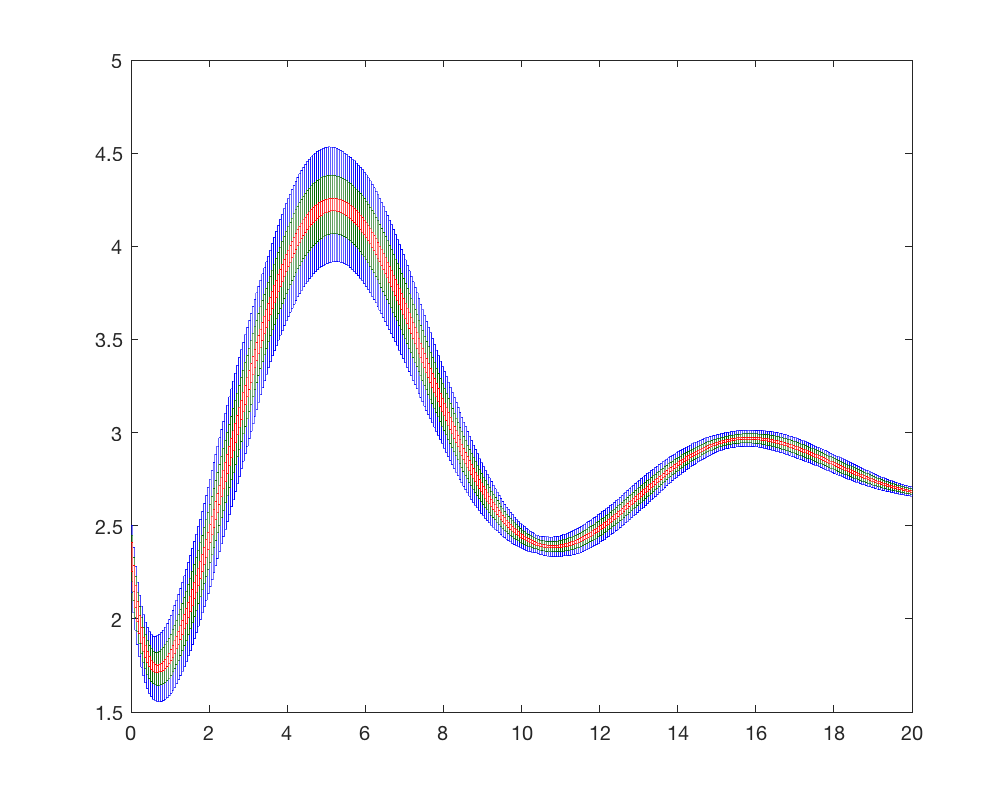
\includegraphics[width=10cm, height=5cm]{../results_flowstar/laub_loomis.png}
  \caption{Flow* (width $w \in 0.01, 0.05, 0.1$)}
\end{figure}
\end{frame}

\begin{frame}{Good: Nonlinear Set Representations}
\begin{figure}[p]
  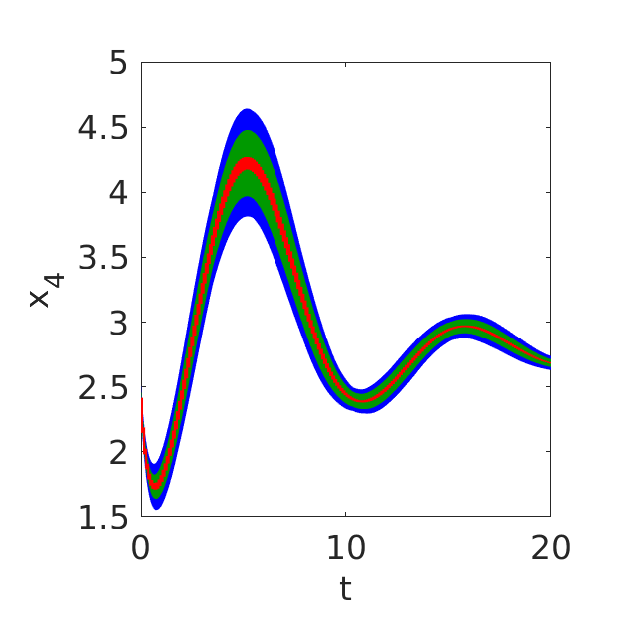
\includegraphics[width=3.5cm, height=3.5cm]{../results_CORA/laubLoomis_27March2019.eps}
  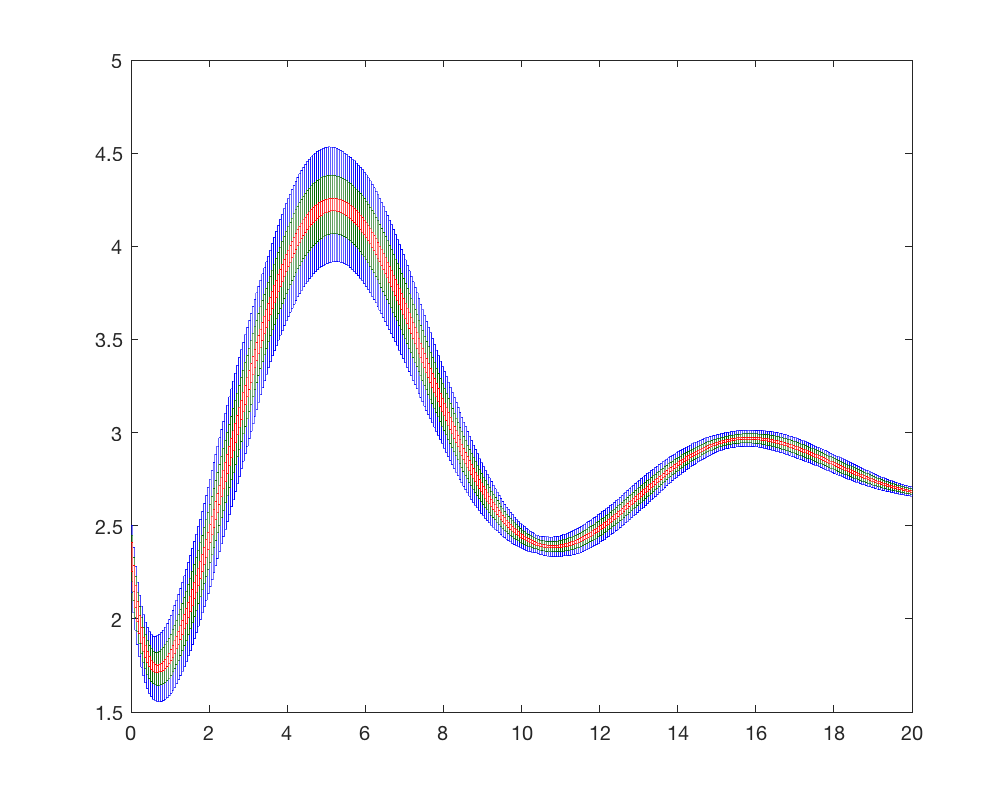
\includegraphics[width=3.5cm, height=3.5cm]{../results_flowstar/laub_loomis.png}
  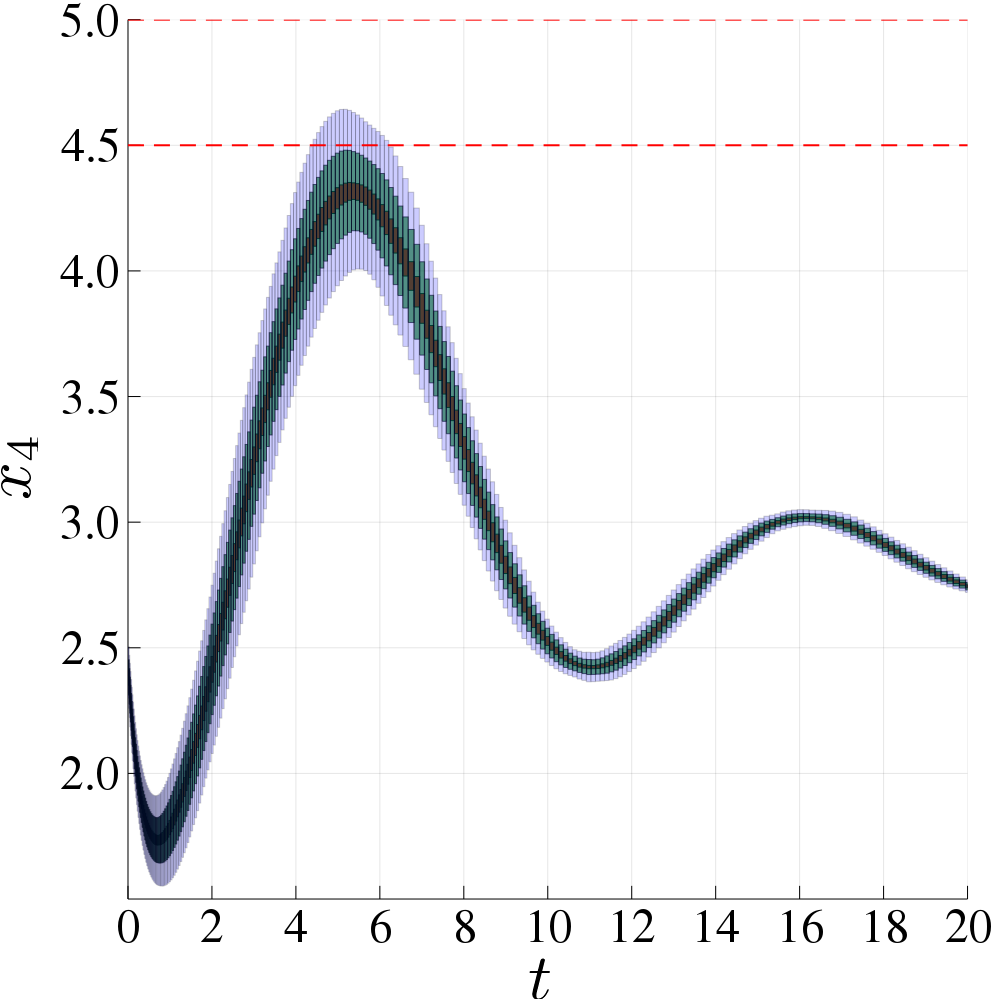
\includegraphics[width=3.5cm, height=3.5cm]{../results_JuliaReach/laubloomis_case_all.png}
  \caption{CORA, Flow*, JuliaReach}
\end{figure}
\small
	\begin{tabular}[c]{lccc}
  \hline
  & \multicolumn{3}{c}{\textbf{computation time in [s]}} \\
  \cmidrule(l){2-4}
  \textbf{tool} & \textbf{$W=0.01$} & \textbf{$W=0.05$} & \textbf{$W=0.1$} \\ \hline
  CORA & $0.82$ & $18$ & $56$  \\
  Flow* & $1.1$ & $2.8$ & $4.9$ \\
  JuliaReach & $3.4$ & $3.3$ & $3.4$ \\
  \hline
\end{tabular}
\end{frame}

\begin{frame}{A Hard Problem}
\begin{figure}[p]
  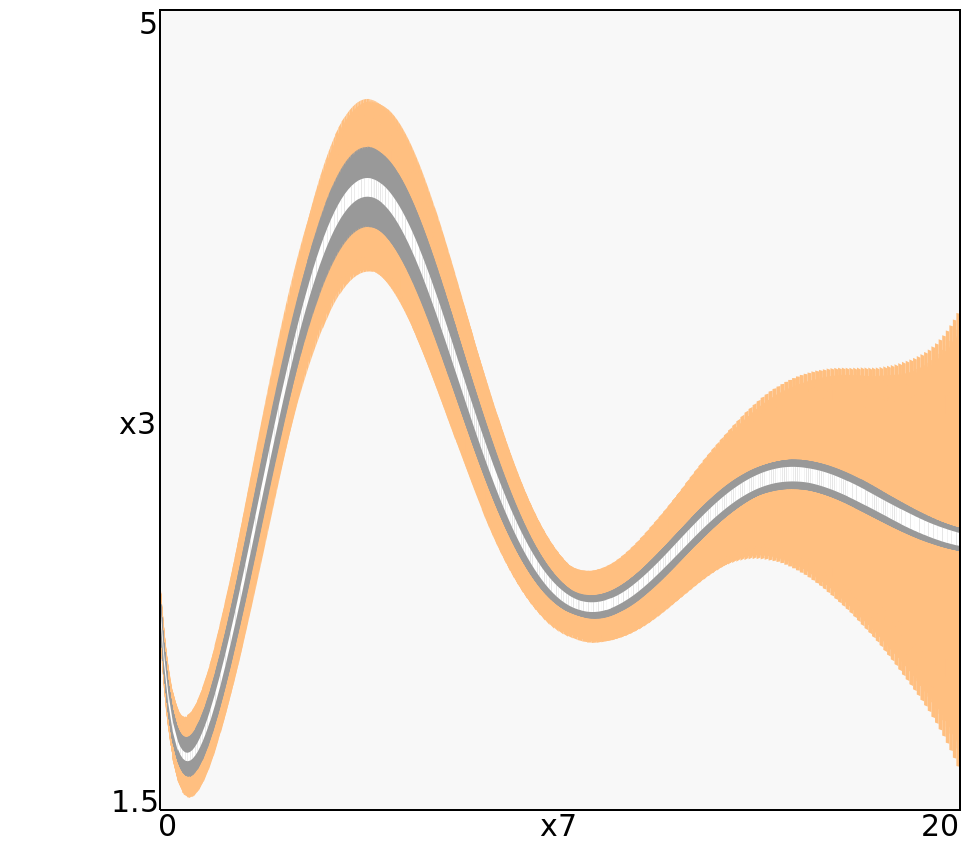
\includegraphics[width=3.5cm, height=3.5cm]{../results_Ariadne/laubloomis.png}
  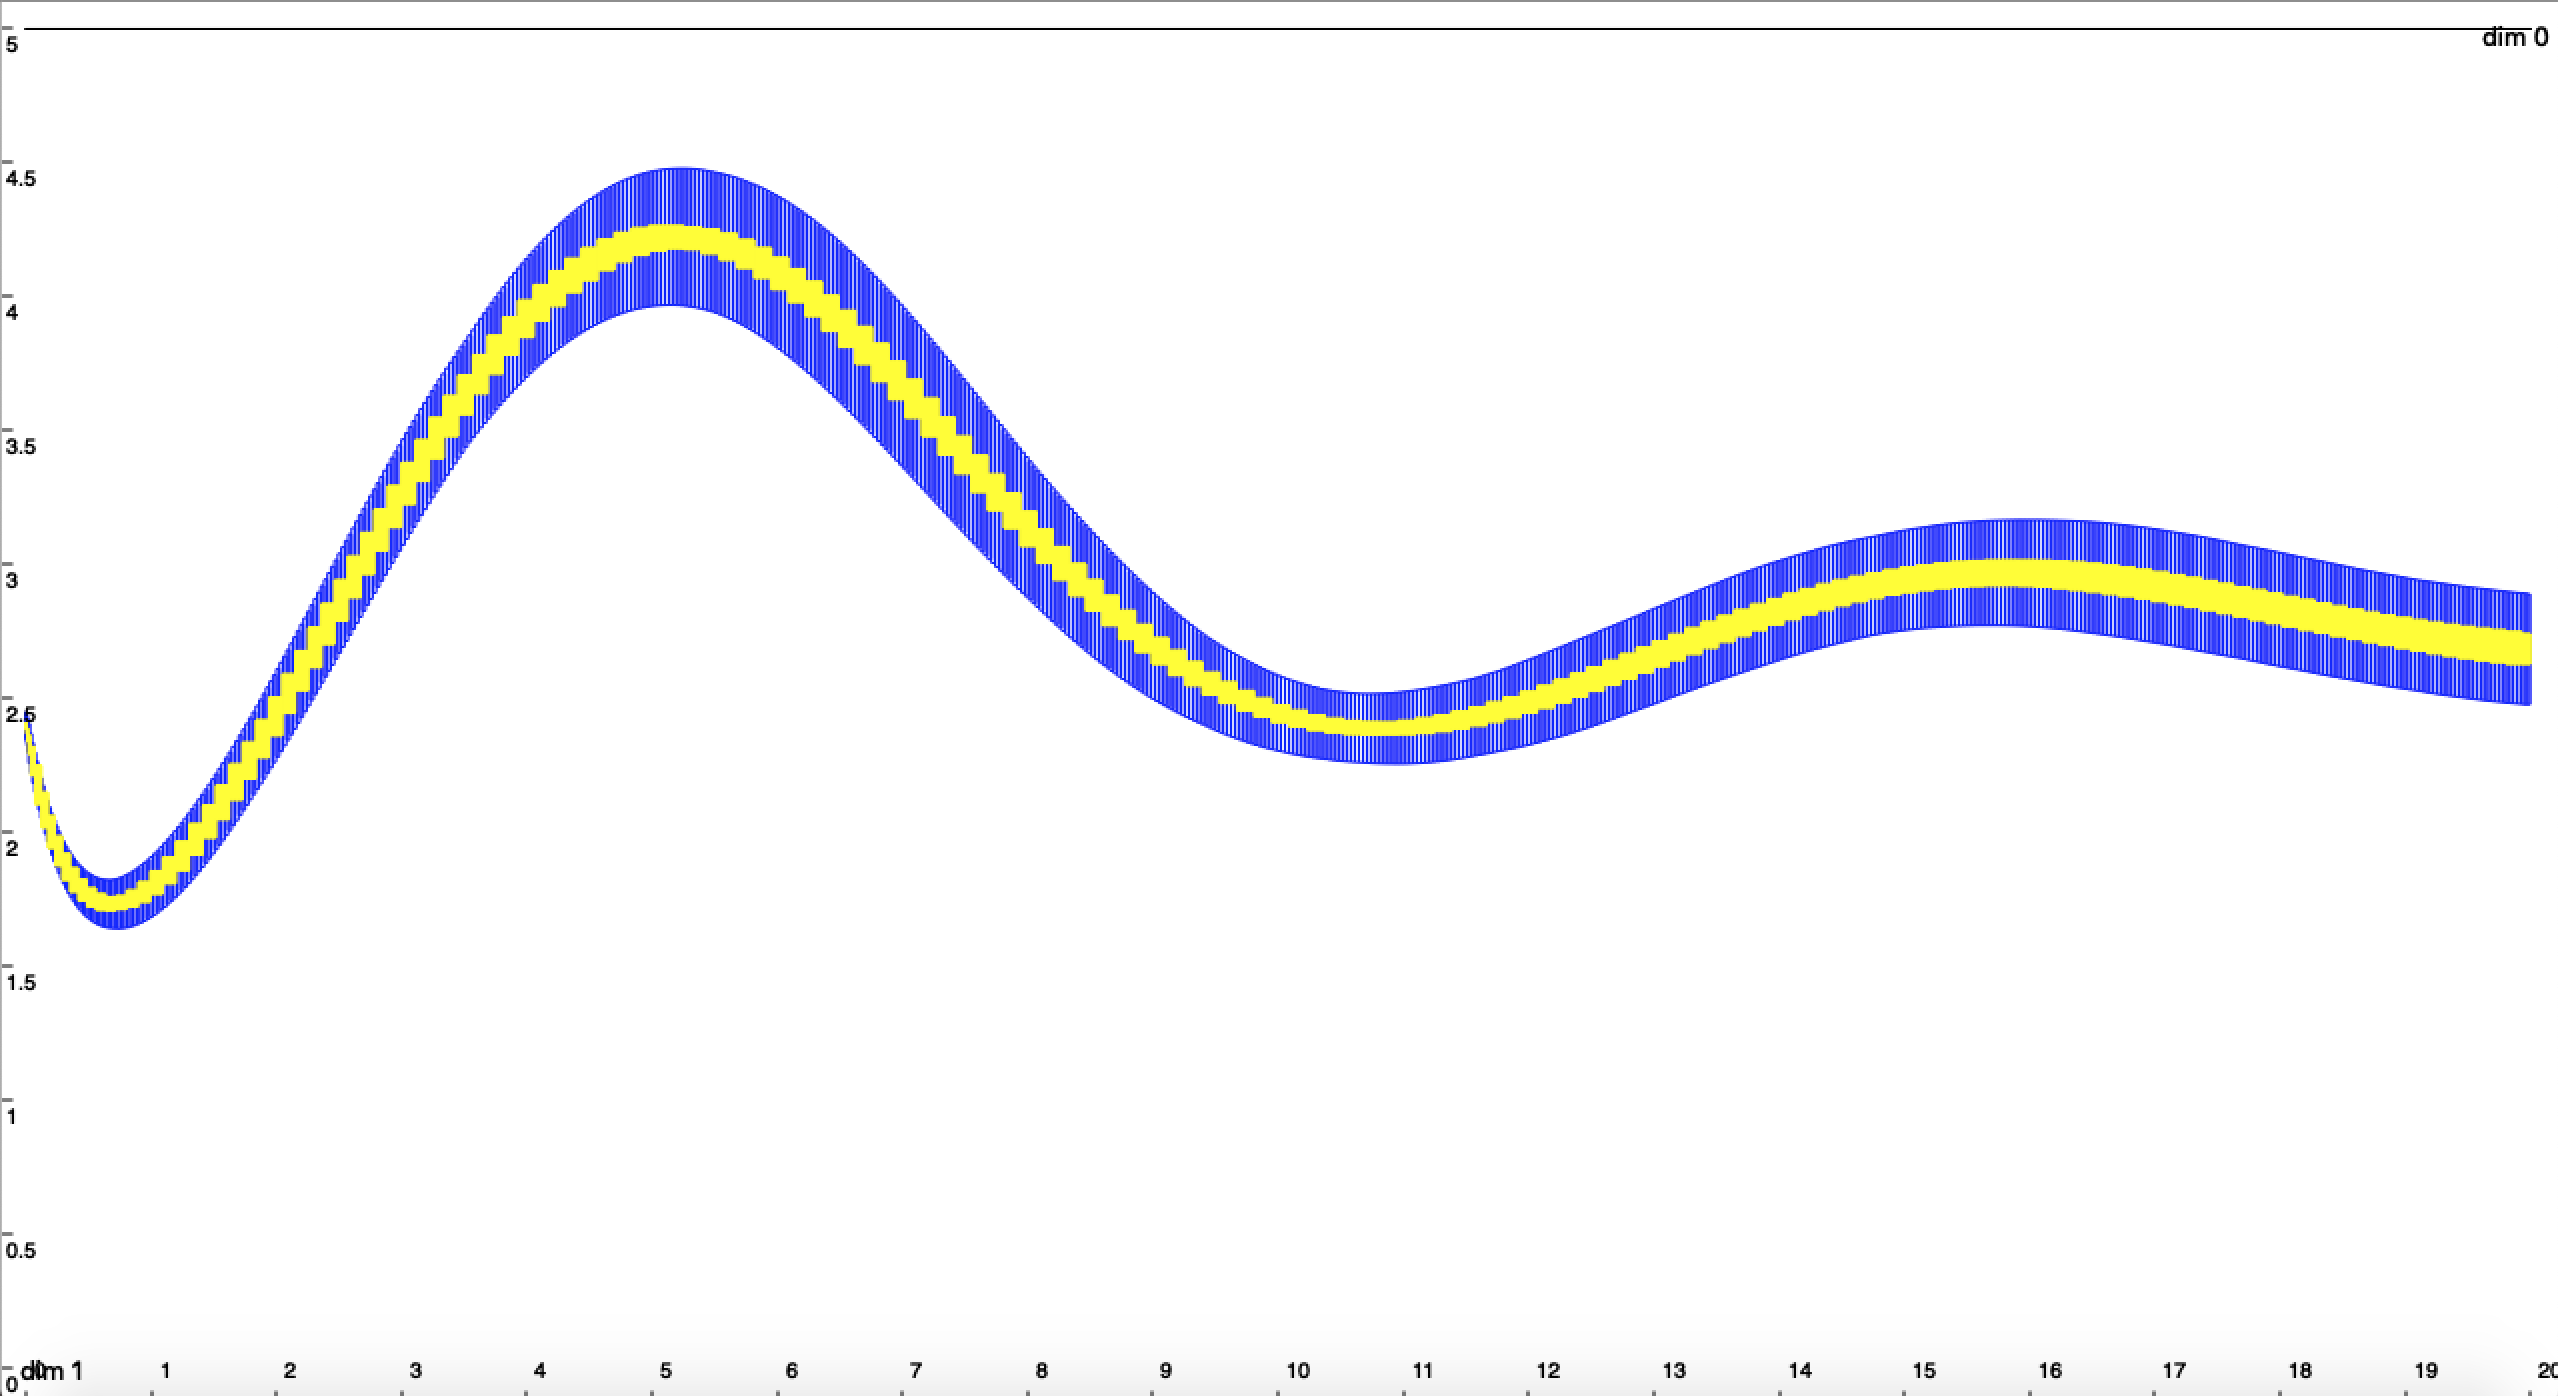
\includegraphics[width=3.5cm, height=3.5cm]{../results_DynIbex/laub-loomis.png}
  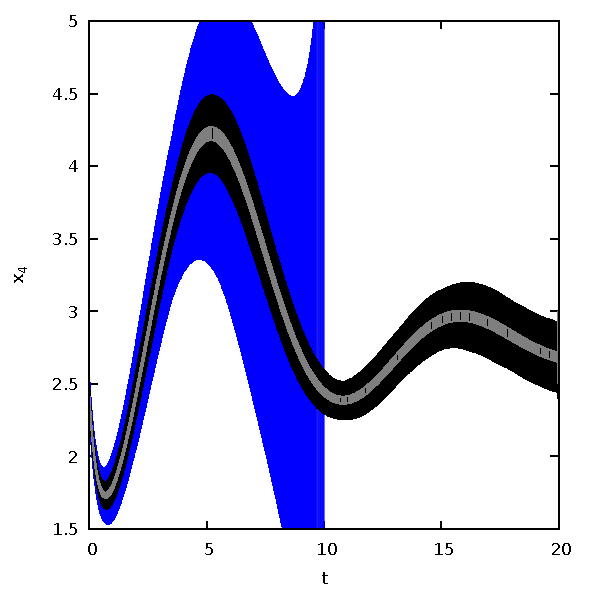
\includegraphics[width=3.5cm, height=3.5cm]{../results_Isabelle/out_ll.pdf}
  \caption{Ariadne(splitting), DynIbex(convex sets, splitting), Isabelle (convex sets, no splitting)}
\end{figure}
\small
\begin{tabular}[c]{lccc}
  \hline
  & \multicolumn{3}{c}{\textbf{computation time in [s]}} \\
  \cmidrule(l){2-4}
  \textbf{tool} & \textbf{$W=0.01$} & \textbf{$W=0.05$} & \textbf{$W=0.1$} \\ \hline
  Ariadne & $7.7$ & $1039$ & $1317$ \\
  DynIbex & $20$ & $64$ & $-$ \\
  Isabelle/HOL & $11$ & $18$ & $-$ \\
  \hline
\end{tabular}
\end{frame}

\begin{frame}{Conclusions}
\begin{itemize}
  \item<+-> three ``old'' tools, three ``new'' tools, three dropped out
  \item<+-> parameter for stiffness of van-der-Pol
    \begin{itemize}
      \item large influence on difficulty
    \end{itemize}
  \item<+-> more initial sets for Laub-Loomis
    \begin{itemize}
      \item shows more precisely when tools get into difficulties
    \end{itemize}
  \item<+-> individual tools
    \begin{itemize}
    \item Flow*: updated module for continuous dynamics (better performance, same/better precision)
    \item Isabelle/HOL: refactoring towards support for (some) standard input format
    \item JuliaReach: last year only in AFF category. Participation fostered international collaboration
  \end{itemize}
\end{itemize}
\end{frame}
\end{document}
